\chapter{Modification of Optical Properties – Controlling Laser Light}
\section{Introduction}
Une bonne question d'examen est \textit{comment changer la polarisation}. On peut parler des matériau
non-isotrope, surface normal, index ellipsoid, \dots\ Une autre bonne question d'examen est 
\textit{Comment modifier une mode}, et ça, c'est l'objectif de ce chapitre. Si on s'intéresse à la
modification d'onde, c'est pour y placer des informations. \\

Nous allons ainsi considérer ici l'effet d'un champ appliqué (magnétique ou électrique) sur la propagation 
d'ondes électromagnétiques dans les cristaux. Dans certains cristaux, la présence d'un champ appliqué va
modifier son index ellipsoid et donc ses modes propres. 

\section{Electro-Optics}
\subsection{Microscopic Theory}
Ce domaine n'existe que depuis une soixantaine d'années car il a fallu attendre l'invention du laser, 
permettant l'obtention de grande puissance optique. Cette grande puissance permettra l'intervention des
ions. On assumera dans ce chapitre que $\vec{\epsilon}$ est modulé à basse fréquence, bien plus petite que celle
de la porteuse, afin de mettre ces ions en mouvement. \\

La susceptibilité dépend des charges liées et de la force avec lesquelles ces électrons sont liés au
noyau. Lorsqu'on applique un champ électrique $\vec{\epsilon}$, les charges liées sont redistribuées et
le réseau ionique est légèrement déformé : le tenseur d'imperméabilité est modifié et, par conséquent, 
les dimension et l'orientation de l'index ellipsoid est modifiée. C'est l'effet \textbf{électro-otpique}. Si
$\vec{\epsilon}$ est petit, on peut développer en série l'imperméabilité
\begin{equation}
\bar{\bar{\eta}}(\epsilon) = \bar{\bar{\eta}}^{(0)}+\bar{\bar{\bar{r}}}.\epsilon + \bar{\bar{\bar{\bar{s}}}}:
\epsilon\epsilon
\label{eq:6.1}
\end{equation}
En notation indicielle
\begin{equation}
\eta_{ij}(\epsilon) = \eta_{ij}^{(0)}+r_{ijk}\epsilon_k+s_{ijkl}\epsilon_k\epsilon_l
\end{equation}
où $\eta_{ij}^{(0)}$ est le tenseur non perturbé donné par
\begin{equation}
\bar{\bar{\eta}} = \left(\begin{array}{ccc}
\frac{1}{n^2_1}&0&0\\
0&\frac{1}{n^2_2}&0\\
0&0&\frac{1}{n^2_3}
\end{array}\right)
\end{equation}
où les constantes $r_{ijk}$ sont les \textbf{coefficients de Pockels}, décrivant les effets électro-optiques
linéaires ($\approx 10^{-12}$ m.V$^{-1}$). Souvent, ces coefficients sont nuls (si le matériau possède une
centrosymétrie) et le second terme devient dominant.Les constants $s_{ijklm}$ sont les \textbf{coefficients
de Kerr}, décrivant les effets électro-optique quadratiques ($\approx 10^{-15}$ m$^2$.V$^{-2}$). \\

Comme les effets électro-optiques sont liés au mouvement ionique, les coefficients sont indépendants de la
fréquence si le voltage est tel que l'on se situe loin des résonances ioniques. On peut alors considérer
les coefficients de Pockels et Kerr comme \textbf{statiques}.

\subsection{Symmetry Properties of Pockels’ Tensor}
\subsubsection{Kleinmann Convention}
Si le milieu est sans pertes et sans activité optique, son tenseur diélectrique est symétrique. Par 
définition, le tenseur d'imperméabilité doit également l’être dans ces conditions. On en déduit que
le tenseur de Pockels est \textit{invariant} pour une permutation de $i$ et $j$ : on passe de 27 à 
18 composants indépendants ! Pour se simplifier la vie, on va "tabuler" le tenseur d'imperméabilité 
de l'effet Pockels et Kerr selon la \textbf{convention de Kleinmann}
\begin{equation}
\begin{array}{lll}
1&=(11)\\
2&=(22)\\
3&=(33)\\
4&=(23)&=(32)\\
5&=(31)&=(13)\\
6&=(12)&=(21)
\end{array}
\end{equation}
Selon cette convention, on peut \textbf{représenter} le tenseur de Pockels comme un tableau $6\times 3$ 
mais attention ce n'est \textbf{pas} un tenseur (pas question de lui appliquer les propriétés des teneurs)
\begin{equation}
\left(\begin{array}{ccc}
r_{11} = r_{111} & r_{12} = r_{112} & r_{13} = r_{113}\\
r_{21} = r_{221} & r_{22} = r_{222} & r_{23} = r_{223}\\
r_{31} = r_{331} & r_{32} = r_{332} & r_{33} = r_{333}\\
r_{41} = r_{231} & r_{42} = r_{232} & r_{43} = r_{233}\\
r_{51} = r_{311} & r_{52} = r_{312} & r_{53} = r_{313}\\
r_{61} = r_{121} & r_{62} = r_{122} & r_{63} = r_{123}
\end{array}\right)
\end{equation}

\newpage
\subsubsection{Principe de Neumann}
On peut encore réduire le nombre de composants indépendants du tenseur de Pockels à l'aide du 
principe de Neumann :
\begin{center}
\textit{Les éléments de symétrie de tout tenseur associé à une propriété matérielle d'un cristal doivent inclure toutes les propriétés de symétrie du groupe de points du cristal.}
\end{center}
Si ce principe est d'application, on en tire que
\begin{equation}
r_{ijk}' = r_{ijk}
\end{equation}
Ce principe démontre la non-présence de l'effet Pockels pour les matériaux centro-symétriques. L'inversion
spatiale pour un tenseur du troisième rang s'écrit 
\begin{equation}
r_{ijk}' = -r_{ijk}
\end{equation}
Selon le principe de Neumann ($r_{ijk}' = r_{ijk}$), on en tire
\begin{equation}
r_{ijk}=0
\end{equation}

\subsection{The Linear Electro-Optic Effect}
Soit un cristal couplé lelong de ses axes principaux sur lequel est appliqué un champ électrique. Une
onde EM incidente va "voir" l'anisotropy et les effets dus au champ électrique. On s'intéresse ici à 
ce qui va se passer dans l'onde qui se propage dans le cristal. \\

Pour trouver les propriétés de propagation d'une onde plane monochromatique, il faut connaître le
tenseur d'imperméabilité : on pourra en déduire le système de coordonnée principal et trouver les 
indices principaux (voir \textit{chapitre 1}). Supposons que le tenseur de Pockels soit non-nul : 
on peut négliger les effets quadratiques :
\begin{equation}
\eta_{ij}(\epsilon) = \eta_{ij}^{(0)}+r_{ijk}\epsilon_k
\end{equation}
Il y a beaucoup de termes la dedans. En utilisant cette expression, on peut trouver l'index ellipsoid
\begin{equation}
\left(\dfrac{1}{n^2_1}+r_{1k}\epsilon_{1k}\right)X^2+
\left(\dfrac{1}{n^2_2}+r_{1k}\epsilon_{2k}\right)Y^2+
\left(\dfrac{1}{n^2_3}+r_{1k}\epsilon_{3k}\right)Z^2+ 
2r_{4k}\epsilon_kYZ + 2r_{5k}\epsilon_kZX+2r_{6k}\epsilon_kXY=1
\label{eq:6.11}
\end{equation}
où $1/n_i^2$ sont les valeurs propres du tenseur d'imperméabilité non-perturbé et $\epsilon_k$ les composantes
du champ électrique appliqué (quand $\epsilon_k=0$, on retrouve l'ellipse non-perturbé). On voit apparaître
trois nouveaux termes non-diagonaux : les axes principaux de l'index ellipsoid perturbés ne coïncident pas avec
ceux de la non-perturbée : elle a subit une rotation. Par rotation, on peut donc retrouver les nouveaux axes
principaux. 

\newpage
\exemple{Considérons l'effet électro-optique dans le KDP. Il s'agit d'un cristal $\bar{42}m$ : axe de 
symétrie incorrect quadruple (rotation de $\pi/2$ autour de l'axe suivi d'une réflexion sur un plan
perpendiculaire à l'axe), conventuellement considéré comme l'axe $z$.  On trouve comme tenseur
\begin{equation}
\left(\begin{array}{ccc}
0&0&0\\
0&0&0\\
0&0&0\\
r_{41}&0&0\\
0&r_{41}&0\\
0&0&r_{63}
\end{array}\right)
\end{equation}
où seuls trois coefficient de Pockels sont non-nuls. L'index ellipsoid devient alors
\begin{equation}
\dfrac{1}{n_0^2}X^2+\dfrac{1}{n_0^2}Y^2+\dfrac{1}{n_0^2}Z^2 + 2r_{41}\epsilon_xYZ+2r_{41}\epsilon_y
ZX+2r_{63}\epsilon_zXY=1
\label{eq:6.13}
\end{equation}
	\begin{center}
	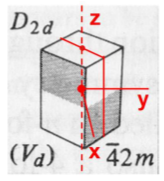
\includegraphics[scale=0.5]{ch6/image1}
	\captionof{figure}{Groupe de symétrie pour le KDP}
	\end{center}

}


\subsubsection{Effet Pockels longitudinal}
Il s'agit du cas où le champ appliqué est parallèle à l'axe de symétrie du cristal
\begin{equation}
\vec\epsilon=\epsilon\vec{1}_z
\end{equation}
L'équation \eqref{eq:6.13} devient
\begin{equation}
\dfrac{X^2+Y^2}{n_0^2}+\dfrac{Z^2}{n_e^2}+2r_{63}\epsilon XY=1
\label{eq:6.15}
\end{equation}
où le dernier terme est \textit{mixte}. Pour étudier les effets, il faut connaître les axes principaux
et les nouveaux indices de réfraction. Pour obtenir la forme standard (sans termes mixtes), il faut effectuer 
une rotation du système autour de l'axe $z$.\\

	\begin{wrapfigure}[6]{l}{5cm}
	\vspace{-5mm}
	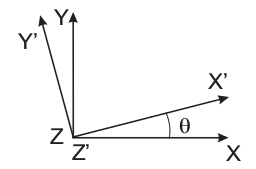
\includegraphics[scale=0.5]{ch6/image2}
	\captionof{figure}{ }
	\end{wrapfigure}
La transformation et son la transformation inverse associée sont données par
\begin{equation}
\left\{\begin{array}{lll}
X' &= X\cos\theta &+ Y\sin\theta\\
Y' &= -X\sin\theta&+ Y\cos\theta\\
Z' &= Z
\end{array}\right.\qquad\qquad
\left\{\begin{array}{lll}
X &= X'\cos\theta &- Y'\sin\theta\\
Y &= X'\sin\theta&+ Y'\cos\theta\\
Z &= Z'
\end{array}\right.
\end{equation}
La substitution dans \eqref{eq:6.15} donne
\begin{equation}
\left(\dfrac{1}{n_0^2}+2r_{63}\epsilon\sin\theta\cos\theta\right)X^{'2}+
\left(\dfrac{1}{n_0^2}-2r_{63}\epsilon\sin\theta\cos\theta\right)Y^{'2}+\dfrac{1}{n_e^2}Z^{'2}+
2r_{63}\epsilon(\cos^2\theta-\sin^2\theta)X'Y'=1
\label{eq:6.18}
\end{equation}
Le terme mixte disparaît si
\begin{equation}
2r_{63}\epsilon(\cos^2\theta-\sin^2\theta)=0\quad\Leftrightarrow\quad \tan\theta=1\quad
\Leftrightarrow\quad\theta=\pm\frac{\pi}{4}
\end{equation}

	\begin{wrapfigure}[12]{r}{4cm}
%	\vspace{-5mm}
	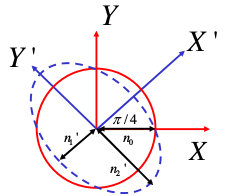
\includegraphics[scale=0.5]{ch6/image3}
	\captionof{figure}{ }
	\end{wrapfigure}
Sous l'application d'un champ électrique, l'index ellipsoid est donc \textbf{tournée de 45$^\circ$} 
par rapport au cas où $\vec{\epsilon}=\vec0$. On peut obtenir les nouveaux indices de réfraction à partir de
\eqref{eq:6.18}
\begin{equation}
n_1' = \left(\dfrac{1}{n_o^2}+r_{63}\epsilon\right)^{-\frac{1}{2}} \approx n_o-\frac{1}{2}n_o^3r_{63}\epsilon
\label{eq:6.20}
\end{equation}
\begin{equation}
n_1' = \left(\dfrac{1}{n_o^2}-r_{63}\epsilon\right)^{-\frac{1}{2}} \approx n_o+\frac{1}{2}n_o^3r_{63}\epsilon
\end{equation}
\begin{equation}
n_3'=n_3=n_e
\end{equation}
La variation des deux indices principaux est proportionnelle aux coefficients de Pockels et au cube de
l'indice ordinaire non-perturbé.



\subsubsection{Effet Pockels transverse}
Considérons cette fois-ci le même cristal KDP (point group $\bar{42}m$) mais avec un champ électrique
appliqué parallèle à l'axe $y$. L'équation \eqref{eq:6.11} devient maintenant
\begin{equation}
\dfrac{X^2+Y^2}{n_o^2}+\dfrac{Z^2}{n_e^2}+2r_{41}\epsilon XZ = 1
\label{eq:6.21}
\end{equation}
Il n'y a ici qu'un terme \textit{mixte} entre $X$ et $Z$ : $y$ reste un axe principal du système et une
rotation autour de cet axe est nécessaire pour retrouver la forme standard de l'index ellipsoid.
\begin{equation}
\left\{\begin{array}{lll}
X&=Z'\sin\theta&+X'\cos\theta\\
Y&=Y'\\
Z&=Z'\cos\theta&-X'\sin\theta
\end{array}\right.
\label{eq:6.22}
\end{equation}
La substitution de \eqref{eq:6.22} dans \eqref{eq:6.21} donne
\begin{equation}
\begin{array}{ll}
&\phantom{+}\DS X^{'2}\left(\dfrac{\cos^2\theta}{n_o^2}+\dfrac{\sin^2\theta}{n_e^2}-r_{41}\epsilon\sin2\theta\right)\vspace{2mm}\\
&+\DS Y^{'2}\left(\dfrac{\sin^2\theta}{n_o^2}+\dfrac{\cos^2\theta}{n_e^2}-r_{41}\epsilon\sin2\theta\right)\vspace{2mm}\\
&+\DS Y^{'2}\left(\dfrac{1}{n_o^2}\right)\vspace{2mm}\\
&+\DS Z'X'\left[\sin2\theta\left(\dfrac{1}{n_o^2}-\dfrac{1}{n_e^2}\right)+2r_{41}\epsilon\left(\cos^2\theta
-\sin^2\theta\right)\right]=1
\end{array}
\end{equation}
Pour faire disparaître le terme mixte, il faut que
\begin{equation}
\tan2\theta=-\dfrac{2r_{41}\epsilon}{\dfrac{1}{n_o^2}-\dfrac{1}{n_e^2}}\qquad\Leftrightarrow\qquad
\theta\approx -\dfrac{r_{41}\epsilon}{\dfrac{1}{n_o^2}-\dfrac{1}{n_e^2}}
\end{equation}
où l'approximation est possible, le coefficient de Pockels étant petit devant 1 et le champ électrique
appliqué est limité pour éviter le claquage. Après quelques manipulations trigonométriques (sans 
approximation)
\begin{equation}
X^{'2}\left(\dfrac{1}{n_o^2}-r_{41}\epsilon\tan\theta\right)+
Z^{'2}\left(\dfrac{1}{n_o^2}+r_{41}\epsilon\tan\theta\right)+
Y^{'2}\left(\dfrac{1}{n_o^2}\right)=1
\end{equation}
On peut en déduire les indices de réfraction. Pour le premier
\begin{equation}
n_1' =\left(\dfrac{1}{n_o^2}-r_{41}\epsilon\tan\theta\right)^{-\frac{1}{2}}\approx
n_o+\frac{1}{2}n_o^3r_{41}\epsilon.\theta
\end{equation}
Comme $\theta\propto \epsilon\to n_i' \propto \epsilon^2$ ce qui n'est pas très pratique : on n'utilise
pas l'effet Pockels transverse en pratique\footnote{La rotation est proportionnelle à la tension appliquée, ce qui est peu pratique (toujours à 45$^\circ$ dans le Pockels longitudinale. L'utilisation de l'effet Pockels transverse nécessite ainsi un système de rétroaction, très difficile à mettre en place.}. De plus, on ne peut utiliser cette approche pour le KDP à 
cause de cette dépendance en $\epsilon^2$ : on ne peut pas négliger les effets NL quadratiques.


\subsection{Polarisation, Amplitude and Phase Modulation}
L'effet Pockels longitudinal permet de modifier la polarisation en $y$. Il est possible de moduler un
signal en appliquant un champ électrique. L'application de celui-ci va faire tourner l'index ellipsoid
de 45$^\circ$. Le champ incident va être projeté dans les nouveaux axes, de façon équitable. Comme
les deux axes sont différents, on va pouvoir induire des retards. 

\subsubsection{Polarisation modulation}
Soit un cristal KDP, un champ appliqué parallèle à $z$ et une onde plane monochromatique polarisée
linéairement selon l'axe $y$ (non-perturbé) se propageant en $z$, incident sur le celui-ci\footnote{Par
exemple avec un polariseur juste avant le cristal}
\begin{equation}
\vec E = E_0e^{i(\omega t-kz))}\vec{1_y}
\end{equation}
Lorsque aucun champ n'est appliqué, cette onde est un mode propre de propagation et il va se propager
sans voir sa polarisation modifiée. Avec un champ électrique appliqué ce n'est plus le cas, mais une 
superposition de deux modes d'indices $n_1'$ et $n_2'$ superposés, donné par \eqref{eq:6.20} \& al. 
\begin{equation}
E(z,t) = \dfrac{E_0}{\sqrt{2}}e^{i\left(\omega t-\frac{\omega}{c}n_1'z\right)}\vec{1_x}+
\dfrac{E_0}{\sqrt{2}}e^{i\left(\omega t-\frac{\omega}{c}n_2'z\right)}\vec{1_y}
\end{equation}
Pour un cristal d'épaisseur $L$, le retard de phase est donné par
\begin{equation}
\begin{array}{ll}
\Gamma &\DS= \left(\omega-\dfrac{\omega}{c}n_1'L\right)-\left(\omega-\dfrac{\omega}{c}n_2'L\right)\vspace{2mm}\\
&\DS=-\dfrac{\omega}{c}L\left(n_o-\dfrac{1}{2}n_o^3r_{63}\epsilon\right)+\dfrac{\omega}{c}L\left(n_o+\dfrac{1}{2}n_o^3r_{63}\epsilon\right)\vspace{2mm}\\
&=\DS\dfrac{\omega}{c}n_o^3r_{63}V = \dfrac{2\pi}{\lambda_0}n_o^3r_{63}V
\end{array}
\end{equation}
Le retard de phase est directement proportionnel à la tension appliquée et donc proportionnel à $\epsilon$. 
Si $\Gamma=\pi$, le rayon qui quitte le cristal est toujours polarisé linéairement, mais tourne de 
$90^\circ$. La tension correspondant à ceci est de
\begin{equation}
V_{pi} = \dfrac{\lambda_0}{2n_o^3r_{63}}
\end{equation}
Celle-ci permet la modulation. Pour un KDP avec $\lambda=632.8$nm, elle vaut $8.4$ kV.


\subsubsection{Modulation en amplitude}
On peut utiliser le même dispositif en plaçant à la fin un analyseur placé orthogonalement au polariseur
d'entrée
\begin{center}
	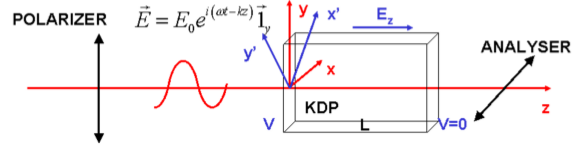
\includegraphics[scale=0.5]{ch6/image4}
	\captionof{figure}{Modulation en amplitude}
\end{center}
La \textit{page 102} reprend le développement de l'onde en sortie, à l'aide des matrices de 
\textsc{Jones} (champ d'entrée, rotation, propagation dans les axes, rotation inverse). On trouve la
même expression de $\Gamma$ que précédemment et comme champ en sortie
\begin{equation}
E_{out} = E_{in}\sin\dfrac{\Gamma}{2}\vec{1_x}
\end{equation}
Il est plus pratique de travailler en intensité
\begin{equation}
I_{out} = \frac{1}{2}\epsilon_0c|E_{out}|^2 = \frac{1}{2}\epsilon_0c E_{in}^2\sin^2\frac{\Gamma}{2}
\end{equation}

	\begin{wrapfigure}[12]{r}{7cm}
	\vspace{-5mm}
	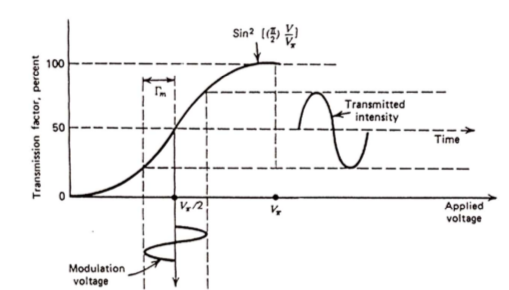
\includegraphics[scale=0.4]{ch6/image5}
	\captionof{figure}{ }
	\end{wrapfigure}
La transmission (représentée ci-contre) est donnée par
\begin{equation}
T \equiv \dfrac{I_{out}}{I_{in}} = \sin^2\left(\dfrac{\pi}{2}\dfrac{V}{V_\pi}\right)
\end{equation}
A cause de la non-linéarité de cette courbe, de nouvelles harmoniques peuvent être créées. Pour 
limiter celles-ci, on va travailler proche du point d’inflexion en $\pi/2$ (par l'application 
d'un tension de biais ou avec une lame $\lambda/4$.). Avec cette disposition, la transmission totale
est donnée par
\begin{equation}
T = \dfrac{1}{2}\left[1+\sin\left(\pi\dfrac{V_m}{V_\pi}\sin\omega_mt\right)\right]
\label{eq:6.38}
\end{equation}

	\begin{wrapfigure}[12]{l}{7cm}
%	\vspace{-5mm}
	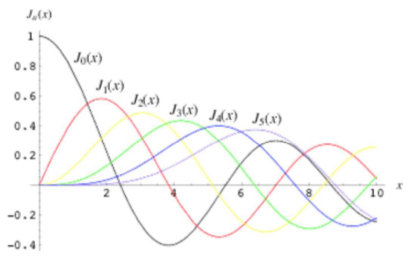
\includegraphics[scale=0.4]{ch6/image6}
	\captionof{figure}{ }
	\end{wrapfigure}
On peut faire apparaître les nouvelles harmoniques en développant la série de Fourier de \eqref{eq:6.38}
\begin{equation}
T = \frac{1}{2}+J_1\left(\pi\dfrac{V_m}{V_\pi}\right)\sin\omega_mt + J_3\left(\pi\dfrac{V_m}{V_\pi}\right)
\sin 3\omega_mt+ \dots
\end{equation}
où $J_i$ sont les fonctions de \textsc{Bessel}. Il semblerait au vue de la précédente expression que 
la bande passante soit infinie. L'amplitude des fonction de \textsc{Bessel} décroît cependant 
rapidement avec l'ordre. Si
\begin{equation}
\pi\dfrac{V_m}{V_\pi} <1
\end{equation}
Toutes les harmoniques sont négligeables et le signal de sortie est une réplique linéaire du signal de
modulation. Si ce n'est pas le cas, le signal de sortie présentera des distorsions.

\newpage
\subsubsection{Modulation en phase}
Le dispositif expérimental est légèrement différent : à la place d'avoir des projections égales sur les
deux axes de biréfringence, le faisceau incident à la polarisation d'un des axes propres afin que sa 
polarisation ne change pas : elle n'est pas retardée\footnote{Lorsqu'on appliquera une tension, on quittera
l'axe propre ce qui causera un saut de phase : modulation.}. L'onde d'entrée est donnée par
\begin{equation}
E(0,t) = E_0e^{i\omega t}\vec{1}_{x'}
\end{equation}
A l'autre bout d'un cristal de longueur $L$
\begin{equation}
\vec E(L,t) = E_0e^ {i\left(\omega t-\dfrac{\omega}{c}n^ {(1)}L\right)}\vec{1_{x'}} = E_0e^{i\left[\omega t-\dfrac{\omega}{c}n_oL+\dfrac{\omega}{2c}n_o^3r_{63}V\right]}\vec{1}_{x'}
\end{equation}
Dans une notation réelle
\begin{equation}
E(L,t) = E_0\cos\left(\omega t-\dfrac{\omega}{c}n_oL+\dfrac{\omega}{2c}n_o^3r_{63}V\right)
\label{eq:6.43}
\end{equation}
En supprimant le terme de phase constante et en appliquant une modulation sinusoïdale du système, on peut
réécrire \eqref{eq:6.43}
\begin{equation}
E_{out} = E_0\cos(\omega t + \beta \sin \omega_mt)
\end{equation}
où $\beta = \frac{\omega n_o^3r_{63}V_m}{2c} = \frac{\pi n_o^ 3r_{63}V_m}{\lambda}$. La porteuse du signal est
donc modulée avec un indice de modulation $\beta$. Pour analyser le contenu spectral, on peut réécrire ce 
signal à l'aide de sa série de Fourier
\begin{equation}
E_{out} = E_0\sum_{n=-\infty}^\infty J_n(\beta)\cos(\omega t + n\omega_mt)
\end{equation}
Il semblerait que la bande passante soit illimitée ce qui n'est pas le cas en pratique (voir \textit{page 106}).
En pratique, la modulation de phase est difficile car on ne peut pas directement mesurer la phase de l'irradiance
du faisceau (il faut un faisceau de référence et procéder par interférence).


\subsection{Comportement à haute fréquence et couplage de modes}
Jusqu'ici nous avions fait l'hypothèse que la phase d'une onde électromagnétique sortant d'un cristal 
électro-optique est déterminée par la valeur instantanée du champ électrique appliqué : ceci n'est plus
vrai si le champ appliqué oscille à haute fréquence (GHz). En effet, celui-ci peut s'annuler/changer
de signe un certain nombre de fois durant le passage de l'onde dans le cristal et le retard de phase 
peut être faible. Il n'est plus question de considérer l'indice de réfraction constant : celui-ci
\textbf{dépend maintenant du temps}.\\

Sans perturbation, les deux modes propres propagations sont bien connus (et possèdent une polarisation
et une vitesse de phase bien connues)\footnote{On utilise $D$ pour ses propriétés mathématiques (toujours
transverse, \dots).}
\begin{equation}
D^{(1)} = A_1e^{i\left(\omega t -\dfrac{\omega}{c}n^{(1)}z\right)}\vec{1}_x,\qquad\qquad
D^{(2)} = A_2e^{i\left(\omega t -\dfrac{\omega}{c}n^{(2)}z\right)}\vec{1}_y
\end{equation}
où nous supposons que l'onde se propage le long d'un des axes principaux du tenseur d'imperméabilité. 
Si le champ électrique varie le long du cristal, on ne peut plus parlé de "mode propre" par définition.
En supposant que la perturbation est petite, on va continuer avec les mêmes modes propres mais avec 
des amplitudes dépendant du temps et de l'espace
\begin{equation}
D^{(1)} = A_1(r,t)e^{i\left(\omega t -\dfrac{\omega}{c}n^{(1)}z\right)}\vec{1}_x,\qquad\qquad
D^{(2)} = A_2(r,t)e^{i\left(\omega t -\dfrac{\omega}{c}n^{(2)}z\right)}\vec{1}_y
\end{equation}
Par effet Pockels, le tenseur d'imperméabilité est perturbé par l'application d'un champ électrique
\begin{equation}
\eta_{ij} = \eta_{ij}^{(0)}+\Delta \eta_{ij}(r,t)
\end{equation}


\subsubsection{Coupled Mode Equation}
Comme $n$ n'est plus constant, il faut résoudre à nouveau l'équation d'onde. 
\begin{equation}
\vec \nabla\times(\vec\nabla\times\bar{\bar{\eta}}.\vec{D}) = -\dfrac{1}{c^2}\dfrac{\partial^2D}{\partial t^2}
\end{equation}
La résolution donnera un système d'équations déterminant la dynamique de l'amplitude : on va prendre
nos modes propres et les insérer. \\

Pour la résolution, on va faire une série d'approximations
\begin{itemize}
\item[$\bullet$] La perturbation dépend seulement de la coordonnée en $z$
\begin{equation}
\Delta \eta_{ij}(r,t)=\Delta \eta_{ij}(z,t)
\end{equation}
Cette hypothèse est assez simple à vérifier avec un bon placement des électrodes. Il en résulte que 
l'amplitude des modes ne dépendra que de la coordonnée $z$
\item[$\bullet$] La perturbation est petite : on négligera les terme de second ordre et plus en 
$\Delta \eta_{ij}$.
\item[$\bullet$] Approximation de l'enveloppe lentement variable (SVEA) : l'amplitude varie de 
façon "smooth", c'est-à-dire que la fréquence de la porteuse est élevée par rapport à la fréquence
de l'enveloppe
\begin{equation}
\left|\dfrac{\partial}{\partial z} A_1(z,t)\right| \ll \left|A_1(z,t)\dfrac{\partial}{\partial z} e^{i\left(
\omega t-\dfrac{\omega}{c}n^{(1)}z\right)}\right|
\end{equation}
\end{itemize}

La composante $x$ de l'équation d'onde est donnée par
\begin{equation}
-\dfrac{\partial^2}{\partial z^2}(\eta_{11}D_x+\eta_{12}D_y)=-\frac{1}{c^2}\dfrac{\partial^2D_x}{\partial t^2}
\end{equation}
En utilisant les différentes approximations pour les deux membres, et en faisant de même pour l'équation en $y$
on trouve deux équations différentielles partielles décrivant la dynamique de la fonction amplitude
\begin{equation}
\begin{array}{ll}
\DS\dfrac{\partial A_1}{\partial z}+\dfrac{n^{(1)}}{c}\dfrac{\partial A_1}{\partial t} &=\DS i\dfrac{\omega}{2c}
n^{(1)3}\Delta\eta_{11}A_1+i\dfrac{\omega}{2c}n^{(1)}n^{(2)2}\Delta\eta_{12}A_2^{-i\frac{\omega}{c}\left(
n^{(2)}-n^{(1)}\right)z}\vspace{2mm}\\
\DS\dfrac{\partial A_2}{\partial z}+\dfrac{n^{(2)}}{c}\dfrac{\partial A_2}{\partial t} &=\DS i\dfrac{\omega}{2c}
n^{(2)3}\Delta\eta_{22}A_2+i\dfrac{\omega}{2c}n^{(1)2}n^{(2)}\Delta\eta_{12}A_1^{-i\frac{\omega}{c}\left(
n^{(1)}-n^{(2)}\right)z}
\end{array}
\label{eq:6.59}
\end{equation}
En regardant la première équation, on voit que les variations de $A_1$ dépendent de $A_1$ elle-même mais aussi
de $A_2$ : les équations sont \textbf{couplées} et c'est la grande nouveauté en hautes fréquences. De fait, sous
perturbation, les modes s’influencent entre eux et ne sont plus indépendants. Si le membre de droite est nul, on
retrouve les équations d'une modulation à basse fréquence. Mais ici, même s'il n'y a pas de couplage (second terme 
du membre de droite), on ne retrouve pas les équations de modulation à basse fréquence ! En conclusion, la modulation
HF est toujours plus compliquée que la BF. Pour résoudre ça, il est impératif de donner une CL sur l'état de 
polarisation de l'onde. 



\subsubsection{Modulation de la phase}
Pour moduler la phase, on veut que la polarisation de l'onde optique soit constante : les modes ne doivent pas
être couplés, c'est-à-dire que
\begin{equation}
\Delta \eta_{12}=\Delta \eta_{21}=0
\end{equation}
En considérant que c'est l'effet Pockels qui perturbe le tenseur d'imperméabilité, cela signifie que tous
les $r_{6k}$ doivent être nuls
\begin{equation}
\Delta\eta_{12}=0\quad\Rightarrow\quad r_{12k}\epsilon_k=0\quad\Rightarrow\quad r_{6k}\epsilon_k=0
\end{equation}
Il faut également qu'au moins un des éléments diagonaux de la perturbation soit non nul
\begin{equation}
\Delta \eta_{11}\neq 0 \quad\Rightarrow\quad r_{11k}\epsilon_k\neq0\quad\Rightarrow\quad r_{1k}\epsilon_k\neq0
\end{equation}
Le KDP ne respecte pas ces conditions, mais le LiNbO$_3$ oui. Supposons une onde polarisée selon l'axe $x$
\begin{equation}
D^{(1)} = A_1e^{i\left(\omega t -\dfrac{\omega}{c}n^{(1)}z\right)}\vec{1}_x
\end{equation}
Soit une modulation sinusoïdale dont la fréquence est bien en dessous de la fréquence de résonance ionique
\begin{equation}
\vec\varepsilon=\varepsilon_0\sin\left(\omega_mt-k_mz\right)\vec{1}_x
\end{equation}
La perturbation du tenseur d'imperméabilité est alors
\begin{equation}
\Delta\eta_{11} = r_{11}\epsilon_0\sin(\omega_mt-k_mz)
\end{equation}
A partir de \eqref{eq:6.59}, l'équation de l'amplitude du mode devient
\begin{equation}
\dfrac{\partial A_1}{\partial z}+\dfrac{n^{(1)}}{c}\dfrac{\partial A_1}{\partial t}=i\dfrac{\omega}{2c}
n^{(1)3}r_{11}\epsilon_0\sin(\omega_mt-k_mz)A_1=i\delta\sin(\omega_mt-k_mz)A_1
\end{equation}
"\textit{La résolution n'est à connaître que si vous choisissez ce chapitre}". Après résolution, on trouve
\begin{equation}
A_1(z,t) = C\left(z-\dfrac{c}{n^{(1)}}t\right) e^{-i\dfrac{\delta c}{\omega_m(n^{(1)}-n_m)}\cos(\omega_mt-k_mz)}
\end{equation}
où $C$ est une fonction arbitraire et $n_m = ck_m/\omega_m$. La fonction $C$ peut être déterminée grâce à la 
condition $A_1(0,t)=A_0$. Ceci fait, on en tire le champ de déplacement du signal de sortie
\begin{equation}
D(L,t) = A_0e^{i\left[\omega t-kL+\beta\sin(\omega_mt-\phi)\right]}\vec{1}_x
\end{equation}
Il s'agit d'un signal à phase modulée dont l'indice de modulation est
\begin{equation}
\beta = \delta L \text{sinc}\left[\dfrac{\omega_m}{2c}\left(n_m-n^{(1)}\right)L\right]
\end{equation}
Si $\omega_m=0$, on retrouve le résultat BF. Si l'indice de réfraction du signal de modulation et de la 
porteuse sont égaux, la sinc vaut l'unité et la modulation est maximale. Physiquement, cela correspond 
au cas où les deux ondes interfèrent constructivement. Ici, pour certaines longueurs du cristal, la 
modulation peut totalement disparaître \footnote{Alors que en BF, la force de la modulation dépendait
de la longueur du cristal, ce phénomène n’apparaissait pas (à verifier).} ! La conclusion est que rien
n'est simple en HF. 

\newpage
\subsection{Propriétés de symétries du tenseur de Kerr}
Étudions maintenant le terme du second ordre de \eqref{eq:6.1}
\begin{equation}
\eta_{ij} = \eta_{ij}^{(0)}+s_{ijkl}\epsilon_k\epsilon_l
\end{equation}
Il est à prendre en considération dans les cristaux où le tenseur de Pockels s'annule. Il s'agit du
tenseur statique additionné du tenseur de Kerr.

\subsubsection{Convention de Kleinmann}
Avec un même raisonnement que dans la deuxième section de ce chapitre, on peut montrer que le tenseur de 
Kerr est invariant à la permutation de ses deux premiers indices. On peut aussi montrer que c'est le cas 
pour ses deux derniers
\begin{equation}
s_{ijkl} = s_{jikl} = s_{ijlk} = s_{jilk}
\end{equation}
De base, il s'agit d'un tenseur 3D de rang 4, qui possède $3^4=81$ composantes. Grâce à la symétrie et 
la convention de Kleinmann, pour le tenseur de Pokels, on avait pu écrire $r_{ijk}\to r_{ij}$ donnant
lieu à un tableau $6\times 3$. Pour Kerr, $r_{ijkl}\to r_{ik}$ soit un tableau $6\times6$, à 36 composantes
au lieu de 81. La convention est reprise à la \textit{page 111}.

\subsubsection{Principe de Neumann}
On peut réduire le nombre de composantes indépendantes du tenseur de Kerr via le principe de Neumann qui
renseigne sur lesquelles des 36 composantes sont nulles et s'il existe une relation entre les composantes
restantes. Les \textit{pages 112} et \textit{113} ainsi que le haut de la page \textit{114} donnent des
exemples de "tenseur". A titre d'exemple, voici les coefficients de Kerr en notation contractée pour un
cristal isotropique
\begin{equation}
\left(\begin{array}{cccccc}
s_{11}&s_{12}&s_{12}&0&0&0\\
s_{12}&s_{11}&s_{12}&0&0&0\\
s_{12}&s_{12}&s_{11}&0&0&0\\
0&0&0&\frac{1}{2}(s_{11}-s_{12}) &0&0\\
0&0&0&0&\frac{1}{2}(s_{11}-s_{12})&0\\
0&0&0&0&0&\frac{1}{2}(s_{11}-s_{12})
\end{array}\right)
\end{equation}

\subsection{Effet électro-optique quadratique}
Pour illustrer, on va étudier l'effet Kerr électro-optique sur un milieu optiquement isotropique. On va
alors choisir l'axe $z$ pour la direction du champ électrique appliqué, de sorte à ce que l'index ellipsoid
s'écrive
\begin{equation}
X^2\left(\frac{1}{n^2}+s_{12}\varepsilon^2\right)+Y^2\left(\frac{1}{n^2}+s_{12}\varepsilon^2\right)
+Z^2\left(\frac{1}{n^2}+s_{11}\varepsilon^2\right)=1
\end{equation}
Ici le résultat est immédiat car les axes principaux sont inchangés. Les nouveaux indices de réfractions
sont donnés par
\begin{equation}
n_1' = n_2' = \left(\frac{1}{n^2}+s_{12}\varepsilon^2\right)^{-\frac{1}{2}}\approx n-\dfrac{1}{2}n^3s_{12}\varepsilon^2,
\qquad
n_3' = \left(\frac{1}{n^2}+s_{11}\varepsilon^2\right)^{-\frac{1}{2}}\approx n-\dfrac{1}{2}n^3s_{11}\varepsilon^2
\end{equation}
Un tel matériau devient donc biréfringent lorsqu'il est placé dans un champ électrique statique (alignement 
des dipôles sous l'influence d'un champ électrique).


\newpage
\section{Magnéto-Optique}
\subsection{Rotation de Faraday}
	\begin{wrapfigure}[13]{l}{8cm}
	\vspace{-5mm}
	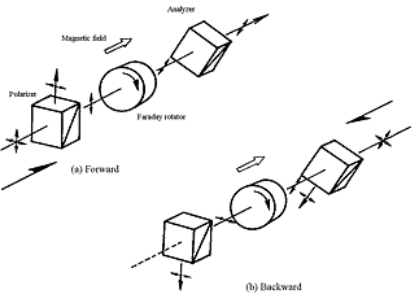
\includegraphics[scale=0.5]{ch6/image7}
	\captionof{figure}{ }
	\end{wrapfigure}
"\textit{Mon effet favori}". Lorsqu'on se propage dans un milieu à activité optique, la polarisation linéaire
ressort avec un angle (par exemple, $+3^\circ$). Si l'on fait le propagation inverse, on va retrouver la propagation 
du début ($+3^\circ-3^\circ=0^\circ$). Ce n'est pas le cas avec l'effet Faraday, car la rotation est indépendante
de la direction de propagation et fonction du champ magnétique d'induction appliqué le long de la distance de 
propagation : la rotation se fera toujours dans le même sens. Supposons une relation linéaire entre le vecteur 
gyration et le champ d'induction magnétique
\begin{equation}
\vec G = \gamma(\vec{B}.\vec{1_k})\vec{1_k}
\end{equation}
Si le vecteur de gyration est suffisamment petit, l'angle de rotation est proportionnel à celui-ci. Dès lors, 
l'angle de rotation est aussi proportionnel au champ magnétique d'induction dan sla direction de propagation
\begin{equation}
\rho = V(\vec{B}.\vec{1}_k)
\end{equation}
où $V$ est la constante de Verdet. Elle est importante dans certains matériaux pour permettre des rotations 
supérieures à $45^\circ$, autorisant la création de "Fadaray rotators", optical isolators\footnote{Les 
back-reflection peuvent déstabiliser un laser.}, \dots 


\subsection{Effet Cotton-Mouton}
Il s'agit d'une perturbation du tenseur diélectrique lorsqu'un champ d'induction magnétique constant est 
appliqué un milieu transparent perpendiculairement à la direction de propagation. C'est un effet du second
ordre et donc l'analogue magnétique de l'effet Kerr. 


\section{Effet Photo-élastique}
Jusqu'ici nous avons vu deux mécanismes pour modifier les propriétés d'une onde électromagnétique
\begin{enumerate} 
\item Via un champ électrique; Pokels et Kerr (pour BF et HF)
\item Via un champ magnétique; Faraday et Cotton-Mouton.
\end{enumerate}
Introduisons une troisième option, celle des déformation mécaniques.\\

Certains matériaux deviennent optiquement non-isotropique lorsqu'on leur applique une tension ou une 
déformation : on parle de photo-élasticité, élasto-optique, stress biréfringence, \dots On peut le décrire
via une relation linéaire entre le tenseur de perméabilité et le tenseur de tension (stress tensor) de 
Cauchy (où l'on néglige les hauts ordres)
\begin{equation}
\eta_{ij} = \eta_{ij}^{(0)}+\pi_{ijkl}\sigma_{kl}
\end{equation}
En assumant la linéarité
\begin{equation}
\eta_{ij} = \eta_{ij}^{(0)}+p_{ijkl}S_{kl}
\end{equation}
où les coefficients $p_{ijkl}$ forment le \textit{strain-optic tensor}. Par la théorie de l'élasticité, on sait
que
\begin{equation}
S_{ii} = \dfrac{\partial u_i}{\partial x_i},\qquad\qquad\qquad
S_{ij} = \dfrac{1}{2}\left(\dfrac{\partial u_i}{\partial x_j}+\dfrac{\partial u_j}{\partial x_i}\right)
\end{equation}
Impliquant que ce tenseur est toujours symétrique.\\

En présence d'un champ de contraintes dans un cristal, l'équation de l'index ellipsoid devient
\begin{equation}
\left(\eta_{ij}^{(0)}+p_{ijkl}S_{kl}\right) x_ix_j=1
\end{equation}
Ce tenseur à les mêmes propriétés qu'un tenseur électro-optique quadratique, on peut à nouveau utiliser la 
convention de Kleinman. Pour un matériau isotropique le \textit{strain-optic tensor} est donné par
\begin{equation}
\left(\begin{array}{cccccc}
p_{11}&p_{12}&p_{12}&0&0&0\\
p_{12}&p_{11}&p_{12}&0&0&0\\
p_{12}&p_{12}&p_{11}&0&0&0\\
0&0&0&\frac{1}{2}(p_{11}-p_{12}) &0&0\\
0&0&0&0&\frac{1}{2}(p_{11}-p_{12})&0\\
0&0&0&0&0&\frac{1}{2}(p_{11}-p_{12})
\end{array}\right)
\label{eq:6.91}
\end{equation}
Une des applications de cet effet est la visualisation des contraintes mécaniques dans les matériaux 
transparents et les \textit{mode scramblers} pour les systèmes de télécom (dispositif qui introduit du couplage 
entre les modes dans une fibre optique). Lire la \textit{page 119} pour les applications. 

\section{Accousto-optique}
La quatrième et dernière méthode se base sur l'effet accousto-optique. Considérons la propagation d'une onde 
longitudinale sonore dans l'eau (direction $z$)
\begin{equation}
u(z,t) = A\cos(\Omega t-Kz)
\end{equation}
où $\Omega$ est utilisé à la place de $\omega$ pour différencier le cas mécanique du cas optique. On retrouve
l'amplitude de l'oscillation $A$, la fréquence sonore $\Omega$ et le nombre d'onde $K$. Cette onde est 
associée à un champ de déformation (strain field) le long de l'axe $z$
\begin{equation}
S_{33}(z,t) = \dfrac{\partial u_z}{\partial z} = KA\sin(\Omega t-Kz)
\end{equation}
Comme l'eau est isotropique, il faut considérer le tenseur optique des contraintes \eqref{eq:6.91}. Comme le
seul coefficient non nul est $S_{33}$, seulement trois composantes du tenseur d'imperméabilité changent
\begin{equation}
\begin{array}{lll}
\Delta \eta_{11} &= p_{1133}S_{33} &= p_{12}KA\sin(\Omega t-Kz)\\
 \Delta \eta_{22} &= p_{2233}S_{33} &= p_{12}KA\sin(\Omega t-Kz)\\
 \Delta \eta_{33} &= p_{3333}S_{33} &= p_{11}KA\sin(\Omega t-Kz)
\end{array}
\end{equation}
La nouvelle index ellipsoid est donnée par
\begin{equation}
\left[\frac{1}{n^2}+p_{12}KA\sin(\Omega t-Kz)\right]x^2+
\left[\frac{1}{n^2}+p_{12}KA\sin(\Omega t-Kz)\right]y^2+
\left[\frac{1}{n^2}+p_{11}KA\sin(\Omega t-Kz)\right]z^2=1
\end{equation}
Les axes principaux ne changent pas, mais le matériau devient non-isotropique
\begin{equation}
n_x=n_y = n-\frac{1}{2}n^3p_{12}KA\sin(\Omega t-Kz),\qquad
n_z = n-\frac{1}{2}n^3p_{11}KA\sin(\Omega t-Kz)
\end{equation}
Les propriétés optiques du milieu sont maintenant inhomogènes et possèdent une périodicité $2\pi/K$ : c'est
analogue à un réseau de Bragg qui se déplace lentement dans l'espace (bien plus lent que la longueur d'onde
de la lumière). \\

Étudions cette approche. Soit une lumière incidente sur le plan $xy$ avec une polarisation selon l'axe $x$. 
On aura des interférences constructives (distance $AOB$) si
\begin{equation}
2\Lambda\sin\theta = m\dfrac{\lambda}{n}
\end{equation}
où $n$ est l'indice non perturbé. Nous avons ici exprimé la condition de Bragg. Si l'onde sonore est 
sinusoïdale, seule le premier ordre ($m=1$) est observé. Comme l'onde électromagnétique est réfléchie par une
onde sonore en mouvement, il va y avoir un décalage Doppler sur la fréquence de l'onde réfléchie. On peut montrer
que ce shift en fréquence vaut
\begin{equation}
\Delta\omega = 2\dfrac{\omega}{c}n\nu \sin\theta = 2\dfrac{2\pi}{\lambda}n\dfrac{\Omega}{2\pi}\Lambda\sin\theta=\Omega
\end{equation}
Soit exactement la fréquence des phonons $\Omega$ ! Ici la description est très classique, mais il y a bien une
interaction photon-phonon. Un approche \textit{quantique avec les mains} est donnée à la page \textit{121}.







\iffalse

Accoustique c'est un peu comme un réseau de bragg : on a une réflexin de bragg
\fi



















